\section{Decision Tree Regression}

I used the DecisionTreeRegressor package from scikitlearn for each of the following plots. 
\begin{figure}[H]
  \centering
  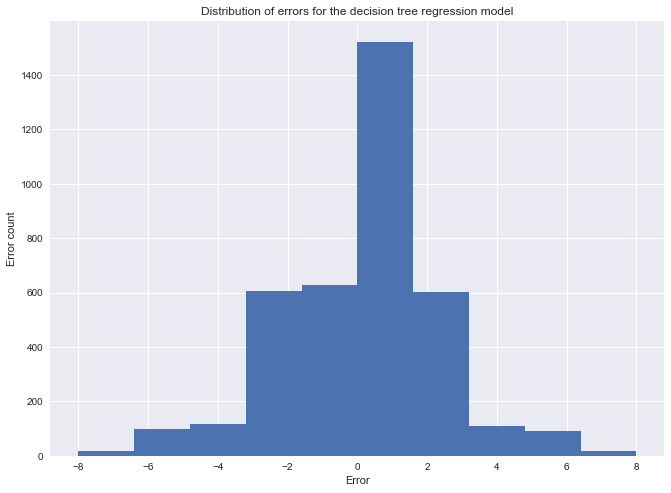
\includegraphics[scale=0.5,width=100mm]{./images/abalone-decision-tree-regression-start.png}
  \caption{Distribution of errors for the decision tree regression model}
  \label{fig:abalone-decision-tree-regression-start}
\end{figure}
Figure \ref{fig:abalone-decision-tree-regression-start} shows the distribution of errors for the decision tree regression model. The results were good with a mean absolute error of 1.64 and standard deviation of the error at 2.229. Without any optimizations of the hyper-parameters decision trees already seem to be a better model than linear regression for predicting the rings of an abalone. To optimize the results I started looking at the hyper-parameters for the DecisionTreeRegressor. To help with the optimization I chose to use RandomizedSearchCV. This enabled me to randomly fit certain hyperparameters using random values without the need for lots of compute power. The results of this optimization can be seen in figure \ref{fig:abalone-decision-tree-regression-randomcv}.
\begin{figure}[H]
  \centering
  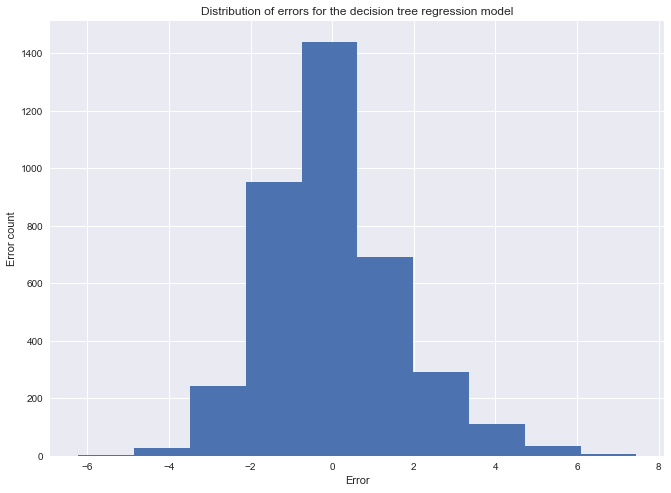
\includegraphics[scale=0.5,width=100mm]{./images/abalone-decision-tree-regression-randomcv.png}
  \caption{Distribution of errors for the decision tree regression model using RandomizedSearchCV}
  \label{fig:abalone-decision-tree-regression-randomcv}
\end{figure}
This is a good improvement. Our mean absolute error went from 1.64 down to 1.257 and the standard deviation of the error went from 2.29 down to 1.64. Visually also, in figure \ref{fig:abalone-decision-tree-regression-randomcv} we can see that the overall histogram is more centred and follows the standard deviation quite well. 
For further optimizations I chose to use GridSearchCV to try and find the best possible result within reason by building on our random values. The grid search took a surprisingly long time to run, initially taking 1 hour. I had to over-clock my computer in order to get this down to 10 minutes. This is probably not recommended for the average computer user, but it does help with speeding up computations. I attempted to look into CUDA to run computations on the GPU\cite{6024507} however due to time constraints I had to drop this line of investigation in order to meet the deadline, however its something I would like to look into in the future. Figure \ref{fig:abalone-decision-tree-regression-gridcv} shows the results. 

\begin{figure}[H]
  \centering
  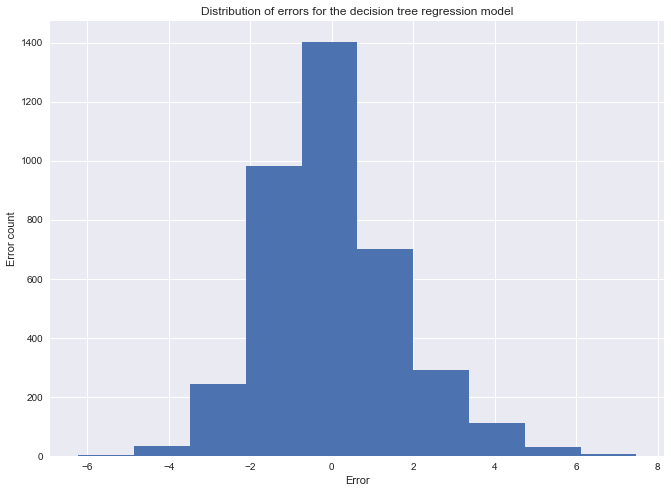
\includegraphics[scale=0.5,width=100mm]{./images/abalone-decision-tree-regression-gridcv.png}
  \caption{Distribution of errors for the decision tree regression model using GridSearchCV}
  \label{fig:abalone-decision-tree-regression-gridcv}
\end{figure}

The grid search marginally improved the mean absolute error, reducing it from 1.257 to 1.255. The standard deviation of the error remained the same with 1.64. The results were a bit disappointing, however given enough time and resources the could probably be reduced further in the future.
Overall, I found decision trees a lot easier to work with than linear regression. I spent a lot of time trying to get linear regression to work and trying to optimize the features for it. I did not have to spend much time at all trying to change any of the data in order for the decision tree to be quite a good predictor.